\documentclass[aspectratio=169]{beamer}

% =================================================================
%  Arrays in C
%  A beginner-friendly Beamer deck (fully self-contained: all
%  figures / diagrams drawn with TikZ, so it compiles anywhere).
%  Style mirrors "c-programming-intro.tex".
% =================================================================

% -------------------------------------------------
% Theme and packages
% -------------------------------------------------
\usetheme{Madrid}
\usecolortheme{default}

\usepackage{amsmath}
\usepackage{amssymb}
\usepackage{bm}
\usepackage{listings}
\usepackage{tikz}
\usepackage{array}
\usepackage{booktabs}
\usepackage{tabularx}
\usepackage{ragged2e}
\usepackage{xcolor}

\usetikzlibrary{shapes.geometric, arrows.meta, positioning, calc, fit, backgrounds}

% -------------------------------------------------
% Colour palette
% -------------------------------------------------
\definecolor{cAccent}{RGB}{0,102,153}     % teal-blue accent
\definecolor{cBox}{RGB}{28,31,42}          % dark box
\definecolor{cGreen}{RGB}{34,139,34}
\definecolor{cRed}{RGB}{178,34,34}
\definecolor{cOrange}{RGB}{204,102,0}
\definecolor{cPurple}{RGB}{102,45,145}
\definecolor{cGrayBg}{RGB}{245,246,248}
\definecolor{codebg}{RGB}{248,248,244}
\definecolor{codekw}{RGB}{0,0,180}
\definecolor{codecomment}{RGB}{0,130,0}
\definecolor{codestr}{RGB}{170,55,20}

% Beamer colour tweaks (match a Madrid-style accent)
\setbeamercolor{structure}{fg=cAccent}
\setbeamertemplate{frametitle continuation}{%
	\ifnum\insertcontinuationcount>1\space(cont...)\fi
}
\setbeamertemplate{navigation symbols}{}
\setbeamertemplate{caption}[numbered]

% -------------------------------------------------
% Listings style for C code
% -------------------------------------------------
\lstdefinestyle{cstyle}{
	language=C,
	backgroundcolor=\color{codebg},
	basicstyle=\ttfamily\footnotesize,
	keywordstyle=\color{codekw}\bfseries,
	commentstyle=\color{codecomment}\itshape,
	stringstyle=\color{codestr},
	numbers=none,
	numberstyle=\tiny\color{gray},
	numbersep=8pt,
	showstringspaces=false,
	breaklines=true,
	frame=single,
	rulecolor=\color{gray!50},
	tabsize=2,
	columns=fullflexible,
	keepspaces=true,
	literate={~}{{$\sim$}}1
}
\lstset{style=cstyle}

% Handy TikZ flowchart node styles
\tikzset{
	startstop/.style={rectangle, rounded corners=10pt, minimum width=2.4cm, minimum height=0.8cm, text centered, align=center, draw=black, fill=cAccent!25},
	process/.style  ={rectangle, minimum width=2.6cm, minimum height=0.8cm, text centered, align=center, text width=2.8cm, draw=black, fill=blue!8},
	io/.style       ={trapezium, trapezium left angle=70, trapezium right angle=110, minimum width=2.2cm, minimum height=0.8cm, text centered, align=center, draw=black, fill=cOrange!20},
	decision/.style ={diamond, aspect=2, minimum width=2.4cm, minimum height=0.9cm, text centered, text width=2.2cm, draw=black, fill=cGreen!18, inner sep=1pt},
	flowarrow/.style={-{Stealth[length=2.5mm]}, thick},
	% array cell helper
	acell/.style={draw=black, minimum width=1.05cm, minimum height=1.0cm, text centered, font=\small, fill=blue!8},
}

\setbeamertemplate{footnote}{%
	\parindent 0em
	\noindent
	\raggedright
	\insertfootnotemark\insertfootnotetext\par
}

% -------------------------------------------------
% Title information
% -------------------------------------------------
\title[Arrays in C]{Arrays in C}
\subtitle{Declaration, Functions, and Multidimensional Arrays}
\author[Amit Kumar Singh]{}
\institute[]{
	Amit Kumar Singh \\
	\vspace{0.1cm}
	Assistant Professor (ECE) \\
	\vspace{0.05cm}
	School of Naval Architecture and Ocean Engineering\\
	\vspace{0.05cm}
	Indian Maritime University Visakhapatnam Campus, Sabbavaram Mandal\\
	\vspace{0.05cm}
	Visakhapatnam, Andhra Pradesh -- 531~035\\
	\vspace{0.25cm}
	amitkumarsingh@imu.ac.in
}
\date[Programming in C]{\today}

\begin{document}

	%------------------------------------------------
	\begin{frame}
		\titlepage
	\end{frame}

	%------------------------------------------------
	\begin{frame}{Outline}
		\small
		\begin{columns}[T,onlytextwidth]
			\hspace{0.8cm}% shift the first column to the right
			\begin{column}{0.49\textwidth}
				\tableofcontents[hideallsubsections, sections={1-4}]
			\end{column}
			\hspace{0.8cm}% wider gap between the two columns
			\begin{column}{0.42\textwidth}
				\tableofcontents[hideallsubsections, sections={5-7}]
			\end{column}
		\end{columns}
	\end{frame}

	% =================================================================
	\section{Introduction to Arrays}
	% =================================================================
	\begin{frame}[fragile]{Why Do We Need Arrays?}
		\begin{block}{The problem}
			Suppose we must store the marks of \textbf{100 students}. With ordinary variables
			we would need 100 separate names --- impossible to write, and a loop cannot help.
		\end{block}
		\begin{columns}[T]
			\begin{column}{0.5\textwidth}
				\centering\textbf{Without arrays}
				\begin{lstlisting}
int m1, m2, m3, /* ... */ m100;
scanf("%d", &m1);
scanf("%d", &m2);
/* ... 100 statements! */
				\end{lstlisting}
				\footnotesize Repetitive, error-prone, and \emph{cannot} be looped.
			\end{column}
			\begin{column}{0.5\textwidth}
				\centering\textbf{With an array}
				\begin{lstlisting}
int marks[100];
for (i = 0; i < 100; i++)
    scanf("%d", &marks[i]);
				\end{lstlisting}
				\footnotesize One name, one loop --- clean and scalable.
			\end{column}
		\end{columns}
		\vspace{0.15cm}
		\centering\footnotesize An \textbf{array} lets many values of the \emph{same} type share \emph{one} name.
	\end{frame}

	\begin{frame}{What is an Array?}
		\begin{block}{Definition}
			An \textbf{array} is a collection of a \textbf{fixed number} of elements of the
			\textbf{same data type}, stored in \textbf{contiguous} memory locations and accessed
			through a common name and an \textbf{index}.
		\end{block}
		\vspace{0.1cm}
		\centering
		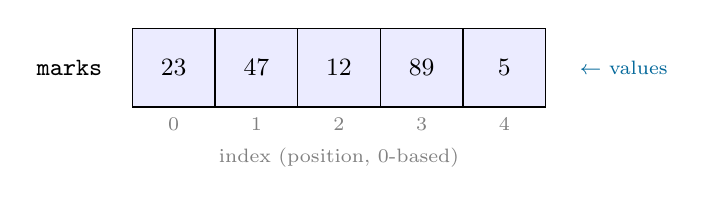
\begin{tikzpicture}
			\foreach \val/\idx in {23/0, 47/1, 12/2, 89/3, 5/4} {
				\node[acell] (c\idx) at (\idx*1.05,0) {\val};
				\node[font=\scriptsize, text=gray] at (\idx*1.05,-0.72) {\idx};
			}
			\node[left=0.25cm of c0, font=\ttfamily\small] {marks};
			\node[right=0.3cm of c4, font=\scriptsize, text=cAccent] {$\leftarrow$ values};
			\node[font=\scriptsize, text=gray] at (2.1,-1.15) {index (position, 0-based)};
		\end{tikzpicture}
		\vspace{0.15cm}
		\begin{itemize}\small
			\item \texttt{marks[0]} is the first element; \texttt{marks[4]} is the last.
			\item The index always starts at \textbf{0} and ends at \textbf{size $-$ 1}.
		\end{itemize}
	\end{frame}

	\begin{frame}{Characteristics of an Array}
		\begin{columns}[T]
			\begin{column}{0.55\textwidth}
				\begin{itemize}
					\item \textbf{Homogeneous} --- all elements share one data type.
					\item \textbf{Fixed size} --- decided when the array is declared.
					\item \textbf{Contiguous} --- elements sit next to each other in memory.
					\item \textbf{Zero-indexed} --- positions run \texttt{0} to \texttt{n-1}.
					\item \textbf{Random access} --- any element is reached directly by its index.
				\end{itemize}
			\end{column}
			\begin{column}{0.45\textwidth}
				\begin{block}{Key idea: random access}
					\small Because elements are contiguous and equally sized, the computer can jump
					straight to \texttt{a[i]} in \emph{one} step --- no need to walk through the others.
				\end{block}
				\begin{block}{The name is an address}
					\small The array name \texttt{a} stands for the address of its first element \texttt{a[0]}.
				\end{block}
			\end{column}
		\end{columns}
	\end{frame}

	% =================================================================
	\section{Declaring Arrays in C}
	% =================================================================
	\begin{frame}[fragile]{Declaring and Initializing Arrays}
		\begin{block}{Syntax}
			\centering \texttt{data\_type\ \ array\_name[size];}
		\end{block}
		\begin{columns}[T]
			\begin{column}{0.55\textwidth}
				\begin{lstlisting}
int   a[5];               /* 5 ints, garbage values */
int   b[5] = {10,20,30,40,50};
int   c[]  = {1, 2, 3};   /* size inferred = 3 */
int   d[5] = {1, 2};      /* rest become 0 */
float temp[7];            /* 7 floats */
char  name[20];           /* holds a string */
				\end{lstlisting}
			\end{column}
			\begin{column}{0.45\textwidth}
				\begin{itemize}\small
					\item The \textbf{size} must be a constant known at compile time.
					\item Fewer initializers than the size $\Rightarrow$ remaining elements are \textbf{0}.
					\item Omitting the size (\texttt{c[]}) lets the compiler \emph{count} the initializers.
				\end{itemize}
				\begin{block}{Beginner trap}
					\small \texttt{int a[5];} gives valid indices \texttt{0..4}. There is \emph{no} \texttt{a[5]}.
				\end{block}
			\end{column}
		\end{columns}
	\end{frame}

	\begin{frame}{Arrays in Memory: Indices and Addresses}
		\begin{block}{Contiguous storage}
			Elements are laid out back-to-back. If each \texttt{int} takes 4 bytes and the array
			starts at address \texttt{1000}, the addresses step by 4.
		\end{block}
		\centering
		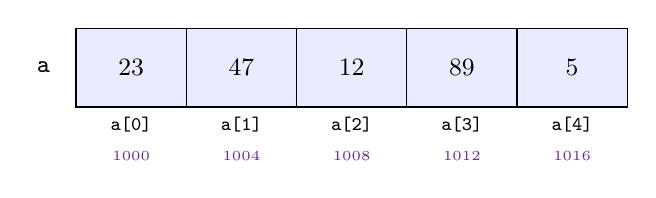
\begin{tikzpicture}
			\foreach \val/\idx/\addr in {23/0/1000, 47/1/1004, 12/2/1008, 89/3/1012, 5/4/1016} {
				\node[acell, minimum width=1.4cm] (c\idx) at (\idx*1.4,0) {\val};
				\node[font=\scriptsize] at (\idx*1.4,-0.72) {\texttt{a[\idx]}};
				\node[font=\tiny, text=cPurple] at (\idx*1.4,-1.12) {\addr};
			}
			\node[left=0.2cm of c0, font=\ttfamily\small] {a};
		\end{tikzpicture}
		\vspace{0.2cm}
		\begin{block}{Address of any element}
			\centering $\&\,\texttt{a[i]} \;=\; \text{base address} \;+\; \texttt{i} \times \texttt{sizeof(type)}$
		\end{block}
		\centering\footnotesize This simple formula is \emph{why} random access costs the same for every index.
	\end{frame}

	\begin{frame}[fragile]{Accessing and Traversing Elements}
		\begin{columns}[T]
			\begin{column}{0.55\textwidth}
				\begin{lstlisting}
int a[5] = {10, 20, 30, 40, 50};
int i;

/* read one element */
printf("%d", a[2]);   /* 30 */

/* walk through every element */
for (i = 0; i < 5; i++)
    printf("%d ", a[i]);
/* prints: 10 20 30 40 50 */
				\end{lstlisting}
			\end{column}
			\begin{column}{0.45\textwidth}
				\begin{itemize}\small
					\item Use the index in square brackets: \texttt{a[i]}.
					\item A \texttt{for} loop with the index \texttt{i} is the natural way to visit every element.
				\end{itemize}
				\begin{block}{Out-of-bounds trap}
					\small C does \textbf{not} check array limits. Writing \texttt{a[5]} or \texttt{a[-1]}
					touches memory you do not own --- a common cause of crashes and bugs.
				\end{block}
			\end{column}
		\end{columns}
	\end{frame}

	% =================================================================
	\section{Passing Arrays to Functions}
	% =================================================================
	\begin{frame}{Passing Arrays to Functions}
		\begin{block}{What actually gets passed}
			An array is \textbf{not copied}. Its name decays to the \textbf{address} of the first
			element, so the function works on the \emph{same} data (``pass by reference''). The
			\textbf{size must be passed separately} --- the function cannot know it otherwise.
		\end{block}
		\vspace{0.1cm}
		\centering
		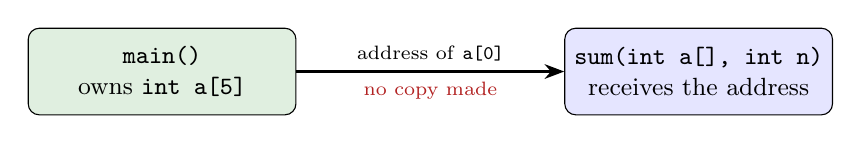
\begin{tikzpicture}[font=\small,
			box/.style={draw, rounded corners, minimum height=1.1cm, align=center, minimum width=3.4cm}]
			\node[box, fill=cGreen!14] (main) {\texttt{main()}\\ owns \texttt{int a[5]}};
			\node[box, fill=blue!10, right=3.4cm of main] (fn) {\texttt{sum(int a[], int n)}\\ receives the address};
			\draw[flowarrow] (main) -- node[above, font=\scriptsize]{address of \texttt{a[0]}}
			node[below, font=\scriptsize, text=cRed]{no copy made} (fn);
		\end{tikzpicture}
		\vspace{0.15cm}
		\begin{itemize}\small
			\item Because there is no copy, a function \emph{can} change the caller's array.
			\item The parameters \texttt{int a[]} and \texttt{int *a} mean the same thing here.
		\end{itemize}
	\end{frame}

	\begin{frame}[fragile]{Example: Sum of an Array}
		\begin{columns}[T]
			\begin{column}{0.58\textwidth}
				\begin{lstlisting}
#include <stdio.h>

/* array decays to a pointer; n = length */
int sum(int a[], int n)
{
    int i, s = 0;
    for (i = 0; i < n; i++)
        s += a[i];
    return s;
}

int main(void)
{
    int marks[5] = {10, 20, 30, 40, 50};
    printf("Total = %d\n", sum(marks, 5));
    return 0;
}
				\end{lstlisting}
			\end{column}
			\begin{column}{0.42\textwidth}
				\begin{block}{How it works}
					\small
					\begin{itemize}
						\item \texttt{sum(marks, 5)} passes the \emph{address} of \texttt{marks} and its length.
						\item Inside, \texttt{a[i]} reads the caller's real data.
						\item We add each element into \texttt{s} and return the total.
					\end{itemize}
				\end{block}
				\centering\footnotesize Output:\; \fbox{\texttt{Total = 150}}
			\end{column}
		\end{columns}
	\end{frame}

	% =================================================================
	\section{Array Applications}
	% =================================================================
	\begin{frame}{Where Are Arrays Used?}
		\begin{columns}[T]
			\begin{column}{0.5\textwidth}
				\begin{block}{Everyday uses}
					\begin{itemize}\small
						\item \textbf{Lists of data} --- marks, prices, temperatures.
						\item \textbf{Strings} --- text is a \texttt{char} array.
						\item \textbf{Tables \& matrices} --- 2-D arrays.
						\item \textbf{Lookup / frequency tables} --- counting how often values occur.
					\end{itemize}
				\end{block}
			\end{column}
			\begin{column}{0.5\textwidth}
				\begin{block}{In algorithms}
					\begin{itemize}\small
						\item \textbf{Searching} --- linear \& binary search.
						\item \textbf{Sorting} --- bubble, selection, insertion.
						\item \textbf{Buffers} --- holding input/output data.
						\item \textbf{Vectors \& polynomials} in maths and graphics.
					\end{itemize}
				\end{block}
			\end{column}
		\end{columns}
		\vspace{0.15cm}
		\centering\footnotesize Almost every non-trivial program stores its data in one or more arrays.
	\end{frame}

	\begin{frame}[fragile]{Application: Frequency Count (Array as a Lookup Table)}
		\begin{columns}[T]
			\begin{column}{0.56\textwidth}
				\begin{lstlisting}
#include <stdio.h>

int main(void)
{
    int digits[10] = {0};   /* ten counters */
    int nums[] = {3, 7, 3, 1, 9, 3, 7};
    int i, n = 7;

    for (i = 0; i < n; i++)
        digits[nums[i]]++;  /* value -> index */

    for (i = 0; i < 10; i++)
        if (digits[i] > 0)
            printf("%d -> %d time(s)\n",
                    i, digits[i]);
    return 0;
}
				\end{lstlisting}
			\end{column}
			\begin{column}{0.44\textwidth}
				\begin{block}{The trick}
					\small The \emph{value} we read is used as an \textbf{index} into the counter array
					--- \texttt{digits[nums[i]]++}. This is a classic, very fast array technique.
				\end{block}
				\centering\footnotesize
				Output:\\[2pt]
				\fbox{\parbox{4cm}{\ttfamily 1 -> 1 time(s)\\ 3 -> 3 time(s)\\ 7 -> 2 time(s)\\ 9 -> 1 time(s)}}
			\end{column}
		\end{columns}
	\end{frame}

	% =================================================================
	\section{Two-Dimensional Arrays}
	% =================================================================
	\begin{frame}{Two-Dimensional Arrays: Tables of Data}
		\begin{block}{Definition}
			A \textbf{2-D array} is an array of arrays --- a grid of \textbf{rows} and \textbf{columns}.
			It is the natural way to store tables, matrices, and images.
		\end{block}
		\begin{columns}[T]
			\begin{column}{0.42\textwidth}
				\centering\vspace{0.1cm}
				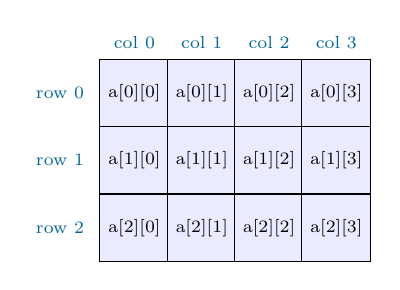
\begin{tikzpicture}[scale=0.9, transform shape,
					gc/.style={draw, minimum size=0.95cm, fill=blue!8, font=\scriptsize}]
					\foreach \row in {0,1,2}
						\foreach \col in {0,1,2,3}
							\node[gc] at (\col*0.95, -\row*0.95) {a[\row][\col]};
					\foreach \col in {0,1,2,3}
						\node[font=\scriptsize, text=cAccent] at (\col*0.95, 0.72) {col \col};
					\foreach \row in {0,1,2}
						\node[font=\scriptsize, text=cAccent] at (-1.05, -\row*0.95) {row \row};
				\end{tikzpicture}
			\end{column}
			\begin{column}{0.58\textwidth}
				\begin{block}{Syntax}
					\centering \texttt{data\_type\ \ name[rows][cols];}
				\end{block}
				\begin{itemize}\small
					\item \texttt{int a[3][4];} is a table of 3 rows $\times$ 4 columns (12 ints).
					\item \texttt{a[i][j]} is the element in \textbf{row i}, \textbf{column j}.
					\item Both indices are 0-based.
				\end{itemize}
			\end{column}
		\end{columns}
	\end{frame}

	\begin{frame}[fragile]{Initializing 2-D Arrays and Row-Major Storage}
		\begin{columns}[T]
			\begin{column}{0.5\textwidth}
				\begin{lstlisting}
int m[2][3] = {
    {1, 2, 3},   /* row 0 */
    {4, 5, 6}    /* row 1 */
};
				\end{lstlisting}
				\footnotesize Even a 2-D array is stored as \textbf{one} straight line in memory ---
				\textbf{row by row} (``row-major'' order).
			\end{column}
			\begin{column}{0.5\textwidth}
				\centering
				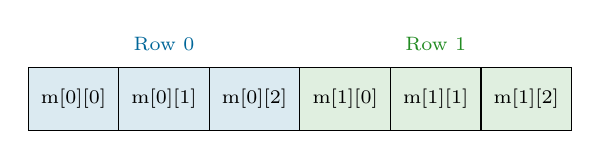
\begin{tikzpicture}[mc/.style={draw, minimum width=1.15cm, minimum height=0.8cm, font=\scriptsize}]
					\foreach \lab/\idx in {m[0][0]/0, m[0][1]/1, m[0][2]/2} {
						\node[mc, fill=cAccent!14] at (\idx*1.15,0) {\lab};
					}
					\foreach \lab/\idx in {m[1][0]/3, m[1][1]/4, m[1][2]/5} {
						\node[mc, fill=cGreen!14] at (\idx*1.15,0) {\lab};
					}
					\node[font=\scriptsize, text=cAccent] at (1.15,0.7) {Row 0};
					\node[font=\scriptsize, text=cGreen] at (4.6,0.7) {Row 1};
				\end{tikzpicture}
				\vspace{0.2cm}
				\footnotesize The address grows left to right: row 0 first, then row 1.
			\end{column}
		\end{columns}
	\end{frame}

	\begin{frame}[fragile]{Traversing a 2-D Array (Nested Loops)}
		\begin{columns}[T]
			\begin{column}{0.55\textwidth}
				\begin{lstlisting}
int m[2][3] = {{1,2,3},{4,5,6}};
int i, j;

for (i = 0; i < 2; i++) {        /* rows */
    for (j = 0; j < 3; j++)      /* cols */
        printf("%d ", m[i][j]);
    printf("\n");                /* new row */
}
				\end{lstlisting}
			\end{column}
			\begin{column}{0.45\textwidth}
				\begin{itemize}\small
					\item The \textbf{outer} loop picks the row; the \textbf{inner} loop picks the column.
					\item Printing a newline after the inner loop lays the output out as a grid.
				\end{itemize}
				\begin{block}{Output}
					\centering\ttfamily 1 2 3\\ 4 5 6
				\end{block}
			\end{column}
		\end{columns}
	\end{frame}

	% =================================================================
	\section{Multidimensional Arrays}
	% =================================================================
	\begin{frame}{Multidimensional Arrays}
		\begin{block}{Beyond two dimensions}
			C allows arrays of \textbf{three or more} dimensions. A 3-D array is like a stack of
			2-D tables --- think of \textbf{pages} in a book, each page a grid.
		\end{block}
		\begin{columns}[T]
			\begin{column}{0.45\textwidth}
				\centering\vspace{0.15cm}
				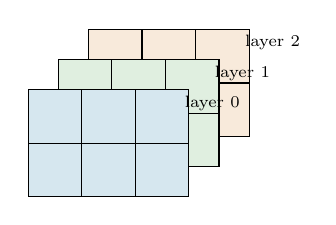
\begin{tikzpicture}[scale=0.85, transform shape]
					\foreach \z/\clr/\lab in {2/cOrange!14/2, 1/cGreen!14/1, 0/cAccent!16/0} {
						\begin{scope}[shift={(\z*0.45,\z*0.45)}]
							\fill[\clr] (0,0) rectangle (2.4,1.6);
							\draw (0,0) rectangle (2.4,1.6);
							\draw (0.8,0) -- (0.8,1.6);
							\draw (1.6,0) -- (1.6,1.6);
							\draw (0,0.8) -- (2.4,0.8);
							\node[font=\scriptsize] at (2.75,1.4) {layer \lab};
						\end{scope}
					}
				\end{tikzpicture}
			\end{column}
			\begin{column}{0.55\textwidth}
				\begin{block}{Declaration \& access}
					\small
					\texttt{int cube[2][3][4];}\\[2pt]
					reserves $2\times3\times4 = 24$ ints.\\[4pt]
					\texttt{cube[k][i][j]} selects \textbf{layer k}, row \texttt{i}, column \texttt{j}.
				\end{block}
				\begin{itemize}\small
					\item Each extra dimension adds one more index and one more nested loop.
					\item In memory it is still \emph{one} contiguous, row-major block.
				\end{itemize}
			\end{column}
		\end{columns}
	\end{frame}

	% =================================================================
	\section{C Program Examples}
	% =================================================================
	\begin{frame}[fragile]{Example 1: Sum and Average of N Numbers}
		\begin{columns}[T]
			\begin{column}{0.62\textwidth}
				\begin{lstlisting}
#include <stdio.h>

int main(void)
{
    int a[100], n, i, sum = 0;

    printf("How many numbers? ");
    scanf("%d", &n);

    for (i = 0; i < n; i++)
        scanf("%d", &a[i]);

    for (i = 0; i < n; i++)
        sum += a[i];

    printf("Sum = %d\n", sum);
    printf("Average = %.2f\n", (float)sum / n);
    return 0;
}
				\end{lstlisting}
			\end{column}
			\begin{column}{0.38\textwidth}
				\begin{block}{Trace for \{10, 20, 30\}}
					\small
					\begin{tabular}{cc}
						\texttt{i} & \texttt{sum} \\ \hline
						0 & 10 \\
						1 & 30 \\
						2 & 60 \\
					\end{tabular}
				\end{block}
				\centering\footnotesize Output:\\ \fbox{\ttfamily Sum = 60}\\[3pt] \fbox{\ttfamily Average = 20.00}
			\end{column}
		\end{columns}
	\end{frame}

	\begin{frame}[fragile]{Example 2: Linear Search}
		\begin{columns}[T]
			\begin{column}{0.58\textwidth}
				\begin{lstlisting}
#include <stdio.h>

int main(void)
{
    int a[] = {5, 8, 12, 3, 19};
    int n = 5, key, i, found = -1;

    printf("Enter value to find: ");
    scanf("%d", &key);

    for (i = 0; i < n; i++) {
        if (a[i] == key) {
            found = i;
            break;
        }
    }

    if (found != -1)
        printf("Found at index %d\n", found);
    else
        printf("Not found\n");
    return 0;
}
				\end{lstlisting}
			\end{column}
			\begin{column}{0.42\textwidth}
				\centering
				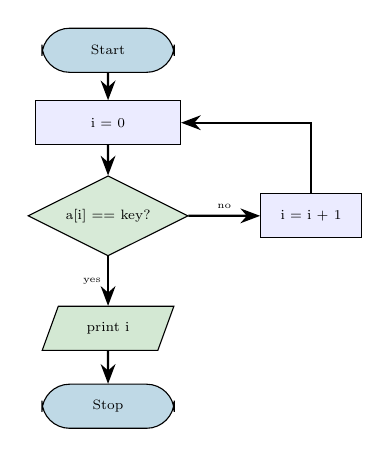
\begin{tikzpicture}[scale=0.7, transform shape,
					font=\scriptsize, node distance=0.5cm]
					\node[startstop] (s) {Start};
					\node[process, below=of s, minimum width=2cm, text width=2.4cm] (init) {i = 0};
					\node[decision, below=0.55cm of init] (c) {a[i] == key?};
					\node[io, below=0.9cm of c, fill=cGreen!20] (yes) {print i};
					\node[process, right=1.3cm of c, minimum width=1.6cm, text width=1.6cm] (inc) {i = i + 1};
					\node[startstop, below=0.6cm of yes] (stop) {Stop};
					\draw[flowarrow] (s) -- (init);
					\draw[flowarrow] (init) -- (c);
					\draw[flowarrow] (c) -- node[left, font=\tiny]{yes} (yes);
					\draw[flowarrow] (c) -- node[above, font=\tiny]{no} (inc);
					\draw[flowarrow] (inc.north) |- (init.east);
					\draw[flowarrow] (yes) -- (stop);
				\end{tikzpicture}
			\end{column}
		\end{columns}
	\end{frame}

	\begin{frame}[fragile]{Example 3: Matrix Addition (2-D Arrays)}
		\begin{columns}[T]
			\begin{column}{0.58\textwidth}
				\begin{lstlisting}
#include <stdio.h>

int main(void)
{
    int A[2][2] = {{1, 2}, {3, 4}};
    int B[2][2] = {{5, 6}, {7, 8}};
    int C[2][2], i, j;

    for (i = 0; i < 2; i++)
        for (j = 0; j < 2; j++)
            C[i][j] = A[i][j] + B[i][j];

    for (i = 0; i < 2; i++) {
        for (j = 0; j < 2; j++)
            printf("%d ", C[i][j]);
        printf("\n");
    }
    return 0;
}
				\end{lstlisting}
			\end{column}
			\begin{column}{0.42\textwidth}
				\begin{block}{The idea}
					\small Add the two matrices \textbf{element by element}: \texttt{C[i][j] = A[i][j] + B[i][j]}
					inside nested loops over rows and columns.
				\end{block}
				\centering\footnotesize
				$\begin{bmatrix} 1 & 2 \\ 3 & 4 \end{bmatrix} +
				 \begin{bmatrix} 5 & 6 \\ 7 & 8 \end{bmatrix} =
				 \begin{bmatrix} 6 & 8 \\ 10 & 12 \end{bmatrix}$
				\\[6pt]
				Output:\; \fbox{\parbox{2.2cm}{\ttfamily 6 8\\ 10 12}}
			\end{column}
		\end{columns}
	\end{frame}

	\begin{frame}{Summary \& What Comes Next}
		\begin{columns}[T]
			\begin{column}{0.5\textwidth}
				\begin{block}{You now know}
					\begin{itemize}\small
						\item Why arrays are needed and what they are.
						\item How to declare, initialize, and traverse arrays.
						\item How arrays sit in memory and how indices map to addresses.
						\item How arrays are passed to functions (by address).
						\item Two-dimensional and multidimensional arrays.
					\end{itemize}
				\end{block}
			\end{column}
			\begin{column}{0.5\textwidth}
				\begin{block}{Practice}
					\begin{itemize}\small
						\item Reverse an array; find its maximum and minimum.
						\item Sort an array (bubble / selection sort).
						\item Multiply two matrices.
					\end{itemize}
				\end{block}
				\begin{block}{Coming up}
					\small Strings (character arrays), pointers, and structures.
				\end{block}
			\end{column}
		\end{columns}
	\end{frame}

	%------------------------------------------------
	\begin{frame}
		\centering
		\Huge Thank You
		\vspace{0.5cm}

		\normalsize Questions?
	\end{frame}

	%------------------------------------------------
\end{document}
